\chapter{Background}
\label{ch:background}

% This chapter provides the fundamental background knowledge that underpins the work included in the thesis. 

Music production techniques related to stereo field are thoroughly rooted in the human perception of sounds, exploiting well-understood auditory phenomena for creative means. However, that understanding is a fairly recent development. In fact, musical practice involving stereophonic sound predated the scientific knowledge of perception by several decades, with one of the earliest known examples dating back the late 19th century \cite{munnTelephoneParisOpera1881}. It wasn't until mid 20th century that the work of \citeauthorandnumber{fletcherLoudnessItsDefinition1933} and \citeauthorandnumber{jeffressPlaceTheorySound1948} outlined the psychoacoustic principles that music production would eventually exploit. In this chapter we draw a line from the basic human physiology of the auditory system, through psychoacoustics, \gls{dsp} theory, and music production, eventually linking them all to the modern computing techniques used as the basis for the work detailed in this thesis. 

\section{The mechanics of hearing and auditory perception}
\label{sec:hearing}

The physical characteristics of the human auditory system govern what we as humans are able to perceive. In particular, our perception of frequency, loudness, and directionality are key when assessing stereo field. 

\subsection{Physiology of the inner ear}
\label{sec:inner_ear}

The ear contains three major sections, loosely labelled the \q{outer}, \q{middle}, and \q{inner} ear (see \cref{fig:ear}). When air vibrations (i.e. sound waves) flow into the outer ear, mechanical coupling in the middle ear transmits vibrations to the cochlea -- the major organ of the inner ear. The cochlea is a conical tube which is coiled up into a spiral, filled with an incompressible fluid, and covered on either end by a membrane. Through the centre of the tube runs the basilar membrane, which is a covered in hairs named cilia. When vibrations are mechanically transmitted to the base of the cochlea, the internal fluid responds by transmitting those vibrations to the basilar membrane, and the cilia will bend and twist accordingly. The cilia are linked to nerve fibres, and will initiate electrical pulses when manipulated. These electrical pulses are sent to the brain and interpreted as sounds \cite{lindsayHumanInformationProcessing1972}.

\begin{figure}[htb]
    \centering
    \resizebox{0.5\textwidth}{!}{
        \begin{tikzpicture}
            \node (pic) at (0,0) {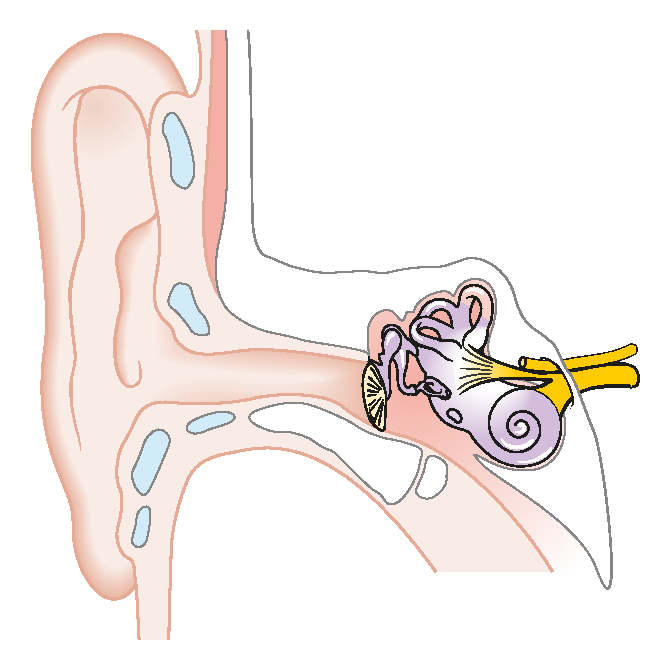
\includegraphics[scale=0.5]{figures/inner_ear.pdf}};
            \node (outer_label) at (-3.5, 0) {Outer ear};
            \node (middle_label) at (0.5, 1.5) {Middle ear};
            \node (inner_label) at (2, 1) {Inner ear};
            \coordinate (outer_point) at (-1.1,-0.4);
            \coordinate (middle_point) at (0.5,-0.1);
            \coordinate (inner_point) at (1.3,-0.5);
            \draw[arrow] (outer_label) -- (outer_point);
            \draw[arrow] (middle_label) -- (middle_point);
            \draw[arrow] (inner_label) -- (inner_point);
        \end{tikzpicture}
    }
    \caption{Diagram of the human ear\textsuperscript{*}. Air flows through the outer ear and vibrates the ear drum. The middle ear mechanically couples the outer ear to the inner ear. The inner ear converts mechanical movements to electrical signals.}
    \label{fig:ear}
    \begin{flushleft}{\scriptsize\textsuperscript{*}\href{https://commons.wikimedia.org/w/index.php?curid=34334173}{Original image} by Cancer Research UK is licensed under \href{https://creativecommons.org/licenses/by-sa/4.0/}{CC BY-SA 4.0}. Annotations have been edited.}\end{flushleft}
\end{figure}

The basilar membrane reacts to a pressure wave from an incoming sound in an elastic way, with a bulge travelling from the base (the widest section) to the apex (the narrowest section). That budge will change amplitude as it travels due to the basilar membrane's non-uniform width and stiffness, and the distance at which is reaches its maximum amplitude depends on the frequency of the incoming sound. Thus, the cilia at different positions along the cochlea have different \q{critical frequencies} that they respond to. The critical frequency increases logarithmically as one moves from the base to the apex, as shown in \cref{fig:cochlea}. The cochlea therefore acts to convert time-domain sound waves into time- and frequency-dependent electrical excitations, enabling us to perceive different frequencies simultaneously. 

\begin{figure}[htb]
    \centering
    \resizebox{\textwidth}{!}{
        
\begin{tikzpicture}
\begin{axis}[
    xmode=log,  
    ymax=2,
    ymin=-0.5,
    xmin=10, 
    xmax=50000, 
    width=\textwidth,
    height=6cm,
    axis x line*=bottom,
    axis y line=none,
    xlabel={Frequency (Hz)},
    xtick={20, 200, 2000, 20000},
    xticklabels={20, 200, 2k, 20k},
]

    \coordinate (base) at (axis cs:20000,0);
    \coordinate (apex) at (axis cs:20,0);
    \coordinate (base_upper) at (axis cs:20000,0.2);
    \coordinate (base_lower) at (axis cs:20000,-0.2);
    \coordinate (apex_upper) at (axis cs:20,0.1);
    \coordinate (apex_lower) at (axis cs:20,-0.1);

    \draw[black] (base_lower) to[bend right=90, looseness=1.618] (base);
    \draw[black] (base) to[bend right=90, looseness=1.618] (base_upper);
    \draw[black] (apex_lower) to[bend left=90, looseness=1.618] (apex_upper);
    \draw[black] (base_upper) -- (apex_upper);
    \draw[black] (base_lower) -- (apex_lower);
    \draw[black, dashed] (base) -- (apex);

    \draw[black,-Latex] (axis cs: 2000, 0.7) node[inner sep=5pt, anchor=south] {Basilar membrane} -- (axis cs: 2000, 0);
\end{axis}

\coordinate (shift) at ($(base) + (0,1.4)$);
\begin{scope}[shift={(shift)}]
\draw[black, densely dotted] plot[smooth, tension=0.618] coordinates {(-0.000,-1.750) (-0.325,-1.688) (-0.627,-1.567) (-0.896,-1.394) (-1.123,-1.178) (-1.302,-0.927) (-1.428,-0.652) (-1.498,-0.363) (-1.512,-0.072) (-1.472,0.212) (-1.380,0.478) (-1.242,0.717) (-1.064,0.922) (-0.855,1.087) (-0.622,1.207) (-0.376,1.280) (-0.125,1.304) (0.122,1.280) (0.356,1.212) (0.568,1.103) (0.753,0.958) (0.904,0.783) (1.018,0.587) (1.090,0.377) (1.122,0.161) (1.112,-0.053) (1.062,-0.258) (0.976,-0.446) (0.859,-0.611) (0.714,-0.749) (0.550,-0.855) (0.371,-0.927) (0.186,-0.963) (-0.000,-0.963) (-0.179,-0.928) (-0.345,-0.862) (-0.493,-0.767) (-0.618,-0.648) (-0.716,-0.510) (-0.786,-0.359) (-0.824,-0.200) (-0.832,-0.040) (-0.810,0.116) (-0.759,0.263) (-0.683,0.394) (-0.586,0.507) (-0.470,0.598) (-0.342,0.664) (-0.207,0.704) (-0.068,0.717) (0.067,0.704) (0.196,0.667) (0.313,0.607) (0.414,0.527) (0.497,0.431) (0.560,0.323) (0.600,0.208) (0.617,0.089) (0.612,-0.029) (0.584,-0.142) (0.537,-0.245) (0.472,-0.336) (0.393,-0.412) (0.302,-0.470) (0.204,-0.510) (0.102,-0.530) (-0.000,-0.530) (-0.098,-0.511) (-0.190,-0.474) (-0.271,-0.422) (-0.340,-0.357) (-0.394,-0.281) (-0.432,-0.197) (-0.453,-0.110) (-0.458,-0.022) (-0.445,0.064) (-0.418,0.145) (-0.376,0.217) (-0.322,0.279) (-0.259,0.329) (-0.188,0.365) (-0.114,0.387) (-0.038,0.395) (0.037,0.388) (0.108,0.367) (0.172,0.334) (0.228,0.290) (0.274,0.237) (0.308,0.178) (0.330,0.114) (0.340,0.049) (0.336,-0.016) (0.321,-0.078) (0.296,-0.135) (0.260,-0.185) (0.216,-0.227) (0.166,-0.259) (0.112,-0.281) (0.056,-0.291) (0.000,-0.291)};
\draw[black, densely dotted] plot[smooth, tension=0.618] coordinates {(-0.000,-1.050) (-0.195,-1.012) (-0.376,-0.940) (-0.537,-0.836) (-0.673,-0.706) (-0.781,-0.556) (-0.856,-0.391) (-0.898,-0.218) (-0.906,-0.043) (-0.881,0.127) (-0.826,0.286) (-0.743,0.429) (-0.637,0.552) (-0.512,0.651) (-0.372,0.722) (-0.225,0.766) (-0.074,0.780) (0.073,0.766) (0.213,0.725) (0.340,0.659) (0.450,0.572) (0.540,0.468) (0.608,0.351) (0.651,0.225) (0.670,0.096) (0.664,-0.032) (0.634,-0.154) (0.583,-0.266) (0.512,-0.365) (0.426,-0.447) (0.328,-0.510) (0.221,-0.553) (0.111,-0.574) (-0.000,-0.574) (-0.107,-0.553) (-0.206,-0.514) (-0.294,-0.457) (-0.368,-0.386) (-0.427,-0.304) (-0.468,-0.214) (-0.491,-0.119) (-0.495,-0.024) (-0.482,0.069) (-0.452,0.156) (-0.406,0.235) (-0.348,0.302) (-0.280,0.356) (-0.204,0.395) (-0.123,0.418) (-0.041,0.426) (0.040,0.419) (0.116,0.396) (0.186,0.360) (0.246,0.313) (0.295,0.256) (0.332,0.192) (0.356,0.123) (0.366,0.053) (0.363,-0.017) (0.347,-0.084) (0.318,-0.145) (0.280,-0.199) (0.233,-0.244) (0.179,-0.279) (0.121,-0.302) (0.060,-0.314) (-0.000,-0.314) (-0.058,-0.302) (-0.112,-0.281) (-0.161,-0.250) (-0.201,-0.211) (-0.233,-0.166) (-0.256,-0.117) (-0.268,-0.065) (-0.271,-0.013) (-0.263,0.038) (-0.247,0.085) (-0.222,0.128) (-0.190,0.165) (-0.153,0.194) (-0.111,0.216) (-0.067,0.229) (-0.022,0.233) (0.022,0.229) (0.064,0.216) (0.101,0.197) (0.134,0.171) (0.161,0.140) (0.182,0.105) (0.195,0.067) (0.200,0.029) (0.198,-0.009) (0.189,-0.046) (0.174,-0.079) (0.153,-0.109) (0.127,-0.133) (0.098,-0.152) (0.066,-0.165) (0.033,-0.171) (0.000,-0.171)};
\draw[black, densely dotted] (0.000,-0.291) to[bend left=90, looseness=1.618] (0.000,-0.171);
\end{scope}

\node[black] at (base) [inner sep=10pt, anchor=west] {Base};
\node[black] at (apex) [inner sep=10pt, anchor=east] {Apex};

\end{tikzpicture}

    }
    \caption{Tonotopic diagram of the human cochlea. Dotted lines represent the cochlea in its normal shape while solid lines show a hypothetical unfurled cochlea with the basilar membrane running down the centre shown as a dashed line. The frequency response of the basilar membrane changes logarithmically along its length, with high frequencies detected at the base and low frequencies at the apex. }
    \label{fig:cochlea}
\end{figure}

\subsection{Directional hearing}
\label{sec:directional_hearing}
\Cref{sec:inner_ear} explains how sound waves are translated in to electrical impulses inside a single ear. When this mechanism is expanded to both ears, combinations of the two sets of electrical impulses can be combined to determine the direction of an incoming sound. 

The psychoacoustic study of spatial hearing has been an active area of research since the mid 20th century, with early examples including the Jeffress model in which time differences between sound events at each ear contribute to a person's ability to locate sounds in space \cite{jeffressPlaceTheorySound1948}. The work of \citeauthor{lindemannEvaluationInterauralSignal1982} a few decades later expanded on this idea by translating the earlier theory to a \gls{dsp} context, and establishing the \gls{ild}, \gls{itd}, and \gls{iacc} as important measures to describe the spatial aspects of binaural signals in a quantifiable way \cite{lindemannEvaluationInterauralSignal1982}.


\begin{figure}[htb]
    \centering
    \resizebox{\textwidth}{!}{
        \begin{tikzpicture}
        \pgfmathsetmacro{\pibyfour}{0.7853981634}
        \pgfmathsetmacro{\ildamp}{0.18}

            % ILD speaker
            \begin{scope}[rotate around={30:(0,0)}]
                \coordinate (speaker_loc) at (4,0);
                \pic[transform shape, scale=0.2] (itd_speaker) at (speaker_loc) {speaker};
                \draw[decorate, decoration={expanding waves, angle=28,segment length=0.4cm}] (speaker_loc) -- (-2,0);
                % \draw[black] (4,0) -- (-4,0);
                \coordinate (shadow_top) at (0,1);
                \coordinate (shadow_middle) at (-2,0);
                \coordinate (shadow_bottom) at (0,-1);
            \end{scope}

            % ILD head
            \fill[lightgray] plot [smooth, tension=1.618] coordinates {(shadow_top) (shadow_middle) (shadow_bottom)};
            \pic[transform shape] (itd_head) at (0,0) {head};
            \node[section_label, minimum width=5.5cm] (itd_label) at (-3, 0) {\glsxtrshort{ild}};

            \begin{scope}[xshift=6cm, yshift=-2cm]
                \begin{axis}[
                    height=6cm, 
                    width=10cm, 
                    ymax=1,
                    ymin=-1,
                    xmin=-1,
                    xmax=11,
                    axis x line=center,
                    axis y line=none,
                    ticks=none,
                    xlabel={time},
                    xlabel style=below right,
                ]
                \addplot[domain=0:10, no markers, smooth] file {generated/ild_L.dat};
                \addplot[domain=0:10, no markers, smooth] file {generated/ild_R.dat};
                \addplot[densely dotted] coordinates {(0, 0.5+\ildamp) (10, 0.5+\ildamp)};
                \addplot[densely dotted] coordinates {(0, 0.5-\ildamp) (10, 0.5-\ildamp)};
                \addplot[densely dotted] coordinates {(0, -0.5+\ildamp*2) (10, -0.5+\ildamp*2)};
                \addplot[densely dotted] coordinates {(0, -0.5-\ildamp*2) (10, -0.5-\ildamp*2)};
                \addplot[latex-latex] coordinates {(-0.2, 0.5+\ildamp) (-0.2, 0.5-\ildamp)};
                \addplot[latex-latex] coordinates {(-0.2, -0.5+\ildamp*2) (-0.2, -0.5-\ildamp*2)};
                \node (a1) at (axis cs: -0.5, 0.5) {$a_L$};
                \node (a2) at (axis cs: -0.5, -0.5) {$a_R$};
                \coordinate (ild_left_y) at (yticklabel cs: 0.75);
                \coordinate (ild_right_y) at (yticklabel cs: 0.25);
                \end{axis}
            \end{scope}

            \node[anchor=east] at (ild_left_y) {Left};
            \node[anchor=east] at (ild_right_y) {Right};


            % ITD 
            \begin{scope}[yshift=-6cm]
                % ITD speaker
                \begin{scope}[rotate around={30:(0,0)}]
                    \coordinate (speaker_loc) at (4,0);
                    \pic[transform shape, scale=0.2] (itd_speaker) at (speaker_loc) {speaker};
                \end{scope}

                % ILD head
                \pic[transform shape] (ild_head) at (0,0) {head};
                \coordinate (left_ear) at (-1.1,0);
                \coordinate (right_ear) at (1.1,0);
                \draw[-Stealth] (speaker_loc) -- (left_ear) node[midway, above] {$d_L$};
                \draw[-Stealth] (speaker_loc) -- (right_ear) node[midway, below] {$d_R$};
                % \node[right] at (4,0) {$d_L > d_R$};
                \node[section_label, minimum width=5.5cm] (itd_label) at (-3, 0) {\glsxtrshort{itd}};

                \begin{scope}[xshift=6cm,yshift=-2cm]
                    \begin{axis}[
                        height=6cm, 
                        width=10cm, 
                        ymax=1.5,
                        ymin=-1,
                        xmin=-1,
                        xmax=11,
                        axis x line=center,
                        axis y line=none,
                        ticks=none,
                        xlabel={time},
                        xlabel style=below right,
                    ]
                    \addplot[domain=0:10, no markers, smooth] file {generated/itd_L.dat};
                    \addplot[domain=0:10, no markers, smooth] file {generated/itd_R.dat};
                    \addplot[densely dotted] coordinates {(\pibyfour 4, 1) (\pibyfour, -1)};
                    \addplot[densely dotted] coordinates {(\pibyfour + 1, 1) (\pibyfour + 1, -1)};
                    \node (tr) at (axis cs: \pibyfour,1.1) {$t_r$};
                    \node (tl) at (axis cs: \pibyfour+1,1.1) {$t_l$};
                    \coordinate (itd_left_y) at (yticklabel cs: 0.6);
                    \coordinate (itd_right_y) at (yticklabel cs: 0.2);
                    \end{axis}
                \end{scope}

                \node[anchor=east] at (itd_left_y) {Left};
                \node[anchor=east] at (itd_right_y) {Right};

            \end{scope}

        \end{tikzpicture}
    }
    \caption{Illustration of how humans perceive the direction of an incoming sound. The physical barrier of the head causes an \glsxtrfull{ild} between sound waves received at the two ears ($a_R-a_L$). The difference in distance from the source to the ears ($d_R - d_L$) causes an \glsxtrfull{itd} between the two ears ($t_l-t_r$).}
    \label{fig:directional_hearing}
\end{figure}

Put simply, we are able to perceive the incoming direction of a sound by observing both the amplitude difference and time difference of coincident sound waves arriving at the left and right ears. Figure \cref{fig:directional_hearing} shows how these two properties enable directional hearing. Firstly, the head itself creates a physical barrier that attenuates sound waves at one ear more-so that at the other ear. Secondly, the difference in distance between the sound source and each ear will create a time delay between the received signals. Over time we learn to associate patterns in \gls{itd}/\gls{ild} with the physical location of the sound source.

The relative importance of \gls{ild} and \gls{itd} differ depending on the frequency of the incoming sound. The reasons for this are twofold. Firstly, a person's inter-aural distance (the physical distance between their ears) must be longer than the wavelength of the incoming sound wave in order for them to detect the phase difference between wave peaks. In this case, it is often referred to as \gls{ipd}, which accounts for the centre frequency of the critical band. Secondly the cilia that line the basilar membrane inside the cochlea can only detect the fine structure of a sound wave up until roughly \qty{1.6}{\kHz} \cite{lindemannEvaluationInterauralSignal1982}. \citeauthor{lindemannEvaluationInterauralSignal1982} gives a rule of thumb that time differences of less than \qty{7.5}{\ms} are heard as a single auditory event (for which direction could be inferred), and differences above \qty{21}{\ms} are heard as uncorrelated events \cite{lindemannEvaluationInterauralSignal1982}. Hence, at \qty{1.6}{\kHz} and below \gls{itd} is more important, whereas above \qty{1.6}{\kHz} \gls{ild} is more important. Furthermore, \citeauthor{blauertSpatialHearingOne1996}'s subsequent work found firstly that both \gls{ild} and \gls{itd} are relevant within the frequency band surrounding \qty{1.6}{\kHz}, and secondly that the angle of incidence of the sound wave plays a role in how the cues are perceived \cite{blauertSpatialHearingOne1996}. Despite this, Lindemann's rules of thumb are still broadly accepted, even being encoded into international standards such as \citetitle{iso-11172-3:mpeg_audio} \cite{iso-11172-3:mpeg_audio}. As an example, \cref{fig:example_pan} shows two recordings (a high-frequency hi-hat and a low-frequency kick drum) that originate from the right-hand side of a listener. The high-frequency hi-hat has a large \gls{ild} and ambiguous \gls{ipd}, whereas the low-frequency kick drum has negligible \gls{ild}, but an interpretable \gls{ipd}.


\begin{figure}[htb]
    \centering
    \includegraphics[scale=0.96]{hihat_kick.pdf}
    \caption{Example sounds coming from the right-hand side, recorded binaurally. High-frequency content (above) has a large \gls{ild} and ambiguous \gls{ipd}, whereas low-frequency content (below) has negligible \gls{ild}, but an interpretable \gls{ipd}.}
    \label{fig:example_pan}
\end{figure}

\subsection{Loudness perception}
While we have established that the \gls{ild} is a key factor of directional hearing, a more detailed understanding of the link between perceived loudness and sound wave intensity is necessary for musical applications.

We perceive the loudness of sound, not in terms of the absolute amplitude of the sound wave, but the \textit{power} of the sound wave. Mathematically speaking, perceived loudness is proportional to the \gls{rms} \gls{spl} raised to an exponent \cite{mooreIntroductionPsychologyHearing2013}. Observing that the calculation of \gls{rms} naturally involves taking the square of the original time function (see \cref{eq:rms_cont,eq:rms_disc} for the continuous and discrete forms respectively), it follows that multiplication of a signal by $\sqrt{2}$ will result in double perceived loudness. Conversely, multiplying a signal by $\frac{1}{\sqrt{2}}$ will halve the perceived loudness.

\begin{align}
    f_{RMS}(t) &= \sqrt{\frac{1}{T_2 - T_1} \int_{T_1}^{T_2}[f(t)^2]dt} \label{eq:rms_cont}\\
    f_{RMS}[n] &= \sqrt{\frac{1}{N}\sum_{n=0}^{N}f[n]^2} \label{eq:rms_disc}
\end{align}

This basic rule is relevant when two sounds are mixed in music production. It defines a precise, mathematical relationship between perceived loudness and the amplification applied by the production equipment or software.

\section{Music production}
\label{sec:music_production}

The principles of our auditory perception have been exploited for creative use since the turn of the 20th century. Early stereophony came from the world of cinema, with sound technicians adding multiple speakers to enable spatial effects\footnote{A typical use case was to match the origin of a voice with the actor's location on the screen.}. Eventually migrating into the music industry, stereophonic recording became the norm in the 1950s \cite{lanierHIFITWOCHANNELCOMMOTION1957,izhakiPanning2023,AbbeyRoadOurStory}. While both cinema and music practitioners have long known that using two speakers for reproduction enabled spatial effects, knowledge of how to \textit{control} those effects came with the psychoacoustic understanding detailed in \cref{sec:hearing}. 


\subsection{Panning}
\label{sec:panning}
The concepts of directional hearing are applied in music production to make sound sources appear as though they originate from a specific direction or position, often referred to as the \q{phantom position}. In recording studio vernacular, this is call \q{panning}. In accordance with the two signal differences a that humans are able to detect (\gls{ild} and \gls{itd}), there are also two basic types of panning -- amplitude panning and time panning. By way of example, \cref{fig:phantom_amplitude} shows how the phantom position can be moved anywhere in between the speakers that are reproducing the sound by applying different amplitude gains to the left and right channel of a stereo recording.

\begin{figure}[htb]
    \centering

    \begin{tikzpicture}
        \def\rad{4};
        \def\expand{1.02};
        \def\soundwaveangle{10};
        \def\soundwavesegmentlength{0.3cm};

        \begin{scope}[rotate around={150:(0,0)}]
            \pic[transform shape, scale=0.2] (left_speaker) at (\rad*\expand,0) {speaker};
        \end{scope}

        \begin{scope}[rotate around={30:(0,0)}]
            \pic[transform shape, scale=0.2] (right_speaker) at (\rad*\expand,0) {speaker};
        \end{scope}
        
        \begin{scope}[rotate around={115:(0,0)}]
            \pic[transform shape, scale=0.2, dotted, line width=0.8pt, line cap=round, dash pattern=on 0pt off 3\pgflinewidth] (phantom_speaker) at (\rad*\expand,0) {speaker};
        \end{scope}

        % labels
        \node[anchor=base east, align=center] (left_label) at (150:\rad+0.9) {Left\\speaker};
        \node[anchor=base west, align=center] (right_label) at (30:\rad+0.9) {Right\\speaker};
        \node[anchor=south west, align=center] (right_label) at (109:\rad+0.5) {Phantom source};

        % Stereo image
        \draw[decorate, decoration={expanding waves, angle=15, segment length=\soundwavesegmentlength}, line width=1.5pt] (115:\rad) -- (0,0);
        \draw[decorate, decoration={expanding waves, angle=10, segment length=\soundwavesegmentlength}, line width=1pt] (150:\rad) -- (0,0);
        \draw[decorate, decoration={expanding waves, angle=5, segment length=\soundwavesegmentlength}, line width=0.5pt] (30:\rad) -- (0,0);

        % Draw full stereo image arc
        \draw (150:\rad) arc (150:30:\rad);

        % Music producer
        \pic (producer) at (0,0) {head};

    \end{tikzpicture}
    \caption{Perception of a phantom sound source created by amplitude panning. The sound wave from the left speaker has higher amplitude than that of the right speaker, thereby creating a phantom source which appears to come from the left.}
    \label{fig:phantom_amplitude}
\end{figure}

Time panning (otherwise known as the \q{Haas effect}) exploits the phenomenon that the first ear to hear a sound generally dictates the direction that it appeared to come from. The process is to simply delay the signal in one channel by a time value within the \q{Haas window} (typically less than 40ms). The undelayed channel will then dictate the phantom direction of the original source. In music production it is used both for panning and to add spaciousness to a recording \cite{stewartWhatHaasEffect2022,izhakiPanning2023}. 

Another frequently used technique is \q{binaural panning}, which assigns combinations of amplitude and time difference to each stereo channel. This is typically achieved by using a \gls{hrir}. An \gls{hrir} is a pair of impulse responses recorded with microphones placed in the ears of either a real person or a dummy head. To obtain an \gls{hrir}, a known excitation signal is played from a specific position in a room and recorded with said binaural microphones (see \cref{fig:phantom_binaural}). The \gls{hrir} can then be convolved with any other monophonic recording to make it appear as though the recording came from the position of the excitation source. An \gls{hrir} can only be used to pan a sound to a single position, so it is typical to record many from different positions \cite{armstrongPerceptualEvaluationIndividual2018}.
%  


\begin{figure}[htb]
    \centering

    \begin{tikzpicture}
        \def\rad{4};
        \def\expand{1.02};
        \def\soundwavesegmentlength{0.4cm};
        \def\yscale{0.8};

        \begin{scope}[rotate around={30:(0,0)}]
            \pic[transform shape, scale=0.2] (right_speaker) at (\rad*\expand,0) {speaker};
        \end{scope}
        
        \draw[lightgray, decorate, decoration={expanding waves, angle=30, segment length=\soundwavesegmentlength}, line width=0.5pt] (30:\rad) -- (0,0);

        % Music producer
        \pic (producer) at (0,0) {head};

        % delta function
        \begin{scope}[xshift=2.2cm, yshift=1.5cm, draw=black]
            \draw[black] (0,0)--(1.26,0);
            \draw[black] (0.05,0)--(0.05,0.7);
            \filldraw[black] (0.05,0.7) circle (1pt);
        \end{scope}
        
        \begin{scope}[xshift=-3cm, yshift=-1cm, draw=black, xscale=0.02, yscale=\yscale]
            \node[minimum width=1.3cm, minimum height=1cm, anchor=west] (left_brir_box) {};
            \draw plot file {generated/brir_L.dat};
        \end{scope}
        \begin{scope}[xshift=1.7cm, yshift=-1cm, draw=black, xscale=0.02, yscale=\yscale]
            \node[minimum width=1.3cm, minimum height=1cm, anchor=west] (right_brir_box) {};
            \draw plot file {generated/brir_R.dat};
        \end{scope}

        \pic[transform shape, scale=0.1, rotate=90, local bounding box=left_mic] (left_mic) at (-1.2,0) {mic};
        \pic[transform shape, scale=0.1, rotate=-90, local bounding box=right_mic] (right_mic) at (1.2,0) {mic};

        \draw[dashed] ([yshift=1pt]left_mic.west) to[out=180, in=60, looseness=1] (left_brir_box.west);
        \draw[dashed] ([yshift=-1pt]left_mic.west) to[out=180, in=30, looseness=1] (left_brir_box.east);
        \draw[dashed] ([yshift=1pt]right_mic.east) to[out=0, in=120, looseness=1] (right_brir_box.east);
        \draw[dashed] ([yshift=-1pt]right_mic.east) to[out=0, in=150, looseness=1] (right_brir_box.west);
        
    \end{tikzpicture}

    \caption{Illustration of a binaural \gls{hrir} being recorded. An impulse is played back through the loudspeaker and recorded at microphones placed in each ear. The head acts a filter, altering the left and right microphone signals differently.}
    \label{fig:phantom_binaural}

\end{figure}


In traditional recording studio setups, the recording engineer or producer will use one or more microphones to capture an original sound source. These singular sound sources are commonly called \q{stems}. During the production process, the stems may be panned to create a sense of space in the final mix. In the case that the stem was recorded using two microphones, the stem would be called a \q{stereo stem}, and the term \q{panning} is usually replaced by \q{balance}, and only amplitude panning (as opposed to time or binaural panning) would be applied.

Amplitude panning is the most common panning technique in traditional music production \cite{shelvockHearingYourAudience2020}. It is associated with so-called \q{panning laws}, which govern how the amplitude is changed in each channel according the desired pan position \cite{izhakiPanning2023}. One example is the \q{energy-preserving pan law} (sometimes called the \mbox{\q{-3dB pan law}}) in which the squared sum of the channel gains always equals 1. The gains of the left and right channel are calculated by $g_L=\cos(\frac{\pi}{2}a)$ and $g_R=\sin(\frac{\pi}{2}a)$ respectively where $a$ is the panning position in the range $[0,1]$. \Cref{fig:equal_power_panning} shows how the channel gains relate to the panning position. The total perceived loudness will be equal at all panning positions.

\begin{figure}[hbt]
    \centering
    \includegraphics[scale=0.85]{equal_power_panning.pdf}\fxwarning[noinline]{Make it so that this diagram is full size but the final sentence still fits on the page.}
    \caption{Channel gains for equal power panning. When both channel gains are $\frac{1}{\sqrt{2}}$, the sound will be centre-panned. The perceived loudness is constant.}
    \label{fig:equal_power_panning}
\end{figure}

Panning techniques are applied to single stems only. A typical recording session will contain multiple stems, each with its own panning.

\subsection{Stereo image}
\label{sec:stereo_image}
The term \q{stereo image} is used to describe the overall distribution of sound across the horizontal plane after panning and any other production techniques have been applied on all stems. One may also use terms like \q{stereo field}, \q{soundstage}, or \q{panorama}, which all refer to the same thing. They are usually described in qualitative terms such as \q{big}, \q{wide}, and \q{ambient} rather than quantitative measures \cite{owsinskiMixingEngineersHandbook2006}. When mixing a musical recording, a producer will pan individual stems to their desired position within the stereo image. Those stems which are recorded in stereo have their own stereo image, which can also be controlled by the producer. The combination of all stems into a final stereo mix constitutes the overall stereo image. 

\Cref{fig:stereo_image} shows a simple example stereo image, as perceived by the producer. It contains two mono stems -- vocals and violin, and one stereo stem -- piano. There are some common tropes seen throughout many productions, some of which are shown in the diagram. Firstly, vocals are recorded in mono and panned to the centre. Secondly, since the piano is panned slightly left, the violin is panned roughly the same amount to the right in order to achieve a balanced mix. Thirdly, all stems are placed in the stereo image in a way that emulates a natural performance on a stage, and to avoid the instruments masking each other. Note that while these practices are commonplace, they are purely an artistic choice on behalf of the producer \cite{owsinskiMixingEngineersHandbook2006}; Recordings breaking the trend are not difficult to find.


\begin{figure}[htb]
    \centering

    \begin{tikzpicture}
        \def\rad{3};
        \def\expand{1.02};

        \begin{scope}[rotate around={150:(0,0)}]
            \pic[transform shape, scale=0.2] (left_speaker) at (\rad*\expand,0) {speaker};
        \end{scope}

        \begin{scope}[rotate around={30:(0,0)}]
            \pic[transform shape, scale=0.2] (right_speaker) at (\rad*\expand,0) {speaker};
        \end{scope}

        % Piano
        \path[fill,lightgray] (0,0) -- (120:\rad)  arc (120:80:\rad) -- (0,0);
        \node at (100:2.2) {Piano};

        % Vocals
        \fill (0,0) (90:\rad) circle (2pt) node[above] {Vocals};

        % Violin
        \fill (0,0) (60:\rad) circle (2pt) node[above right] {Violin};

        % Stereo image
        \path[draw, dashed] (0,0) -- (120:\rad);
        \path[draw, dashed] (0,0) -- (60:\rad);
        \path[draw, dotted] (0,0) -- (150:\rad);
        \path[draw, dotted] (0,0) -- (30:\rad);

        % Draw full stereo image arc
        \draw (150:\rad) arc (150:30:\rad);

        % Music producer
        \pic[scale=0.618] (producer) at (0,0) {head};

    \end{tikzpicture}
    \caption{Example stereo image created by a music producer. Mono stems are shown as black dots and a stereo stem as a grey fill. Dashed lines represent the extent of the stereo image. Dotted lines represent the maximum boundaries of the possible stereo image.}
    \label{fig:stereo_image}
\end{figure}

\subsection{Production equipment and software}

To create a stereo image, a music producer will use the equipment available in a typical recording studio. Before the advent of digital recording, said equipment usually comprised a mixing console where each stem was assigned to one \q{track}. Each track had individual controls for (amongst others) level and panning that were directly linked to the internal electronics. The producers might also use the term \q{fader} for the level control and \q{pan-pot} for the panning control\footnote{The term \q{pan-pot} is a shortening of \q{panoramic potentiometer}.}. All tracks would be mixed by the console and the combined output fed to stereo speakers for playback. In a digital recording studio, the equipment is largely the same except that the mixing console will be connected to a computer that controls the session and stores the recorded audio. \Cref{fig:recording_studio} shows photographs of a small recording studio where the faders and pan-pots for each track are visible. The music producer will manipulate the physical controls for each track to create a stereo mix.

\begin{figure}[hbt]
    \centering
    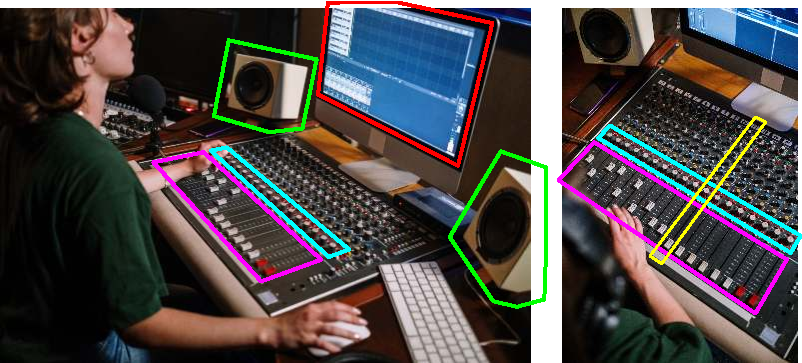
\includegraphics[width=\linewidth] {figures/studio_photos_small.pdf}
    \caption{Photographs of a small recording studio\textsuperscript{*}. The left photo shows all studio equipment, while the right photo shows a close-up of the mixing console. Faders are highlighted pink, pan-pots are highlighted blue, stereo speakers are highlighted green, and the computer running a \glsfmtfull{daw} is highlighted red. One track is highlighted yellow.}
    \label{fig:recording_studio}
    \begin{flushleft}{\scriptsize\textsuperscript{*}\href{https://www.pexels.com/photo/a-person-in-green-crew-neck-t-shirt-sitting-infront-of-computer-and-audio-mixer-5657660/}{Original} \href{https://www.pexels.com/photo/person-using-audio-mixer-5657676/}{images} by cottonbro studio are licensed under \href{https://www.pexels.com/license/}{Pexels}. Annotations have been added.}\end{flushleft}
\end{figure}

In modern recording scenarios a music producer typically uses a \gls{daw} - graphical software that allows them to record and edit audio. There are many \glspl{daw} available, but one such example (Reaper) is shown in \cref{fig:daw}. In particular, it shows a single recorded audio track which has its \q{Pan} control automated. In a more complete recording session, the \gls{daw} would contain many more tracks, each with their own pan control.

\begin{figure}[p!]
    \centering
    \begin{subfigure}[b]{\textwidth}
        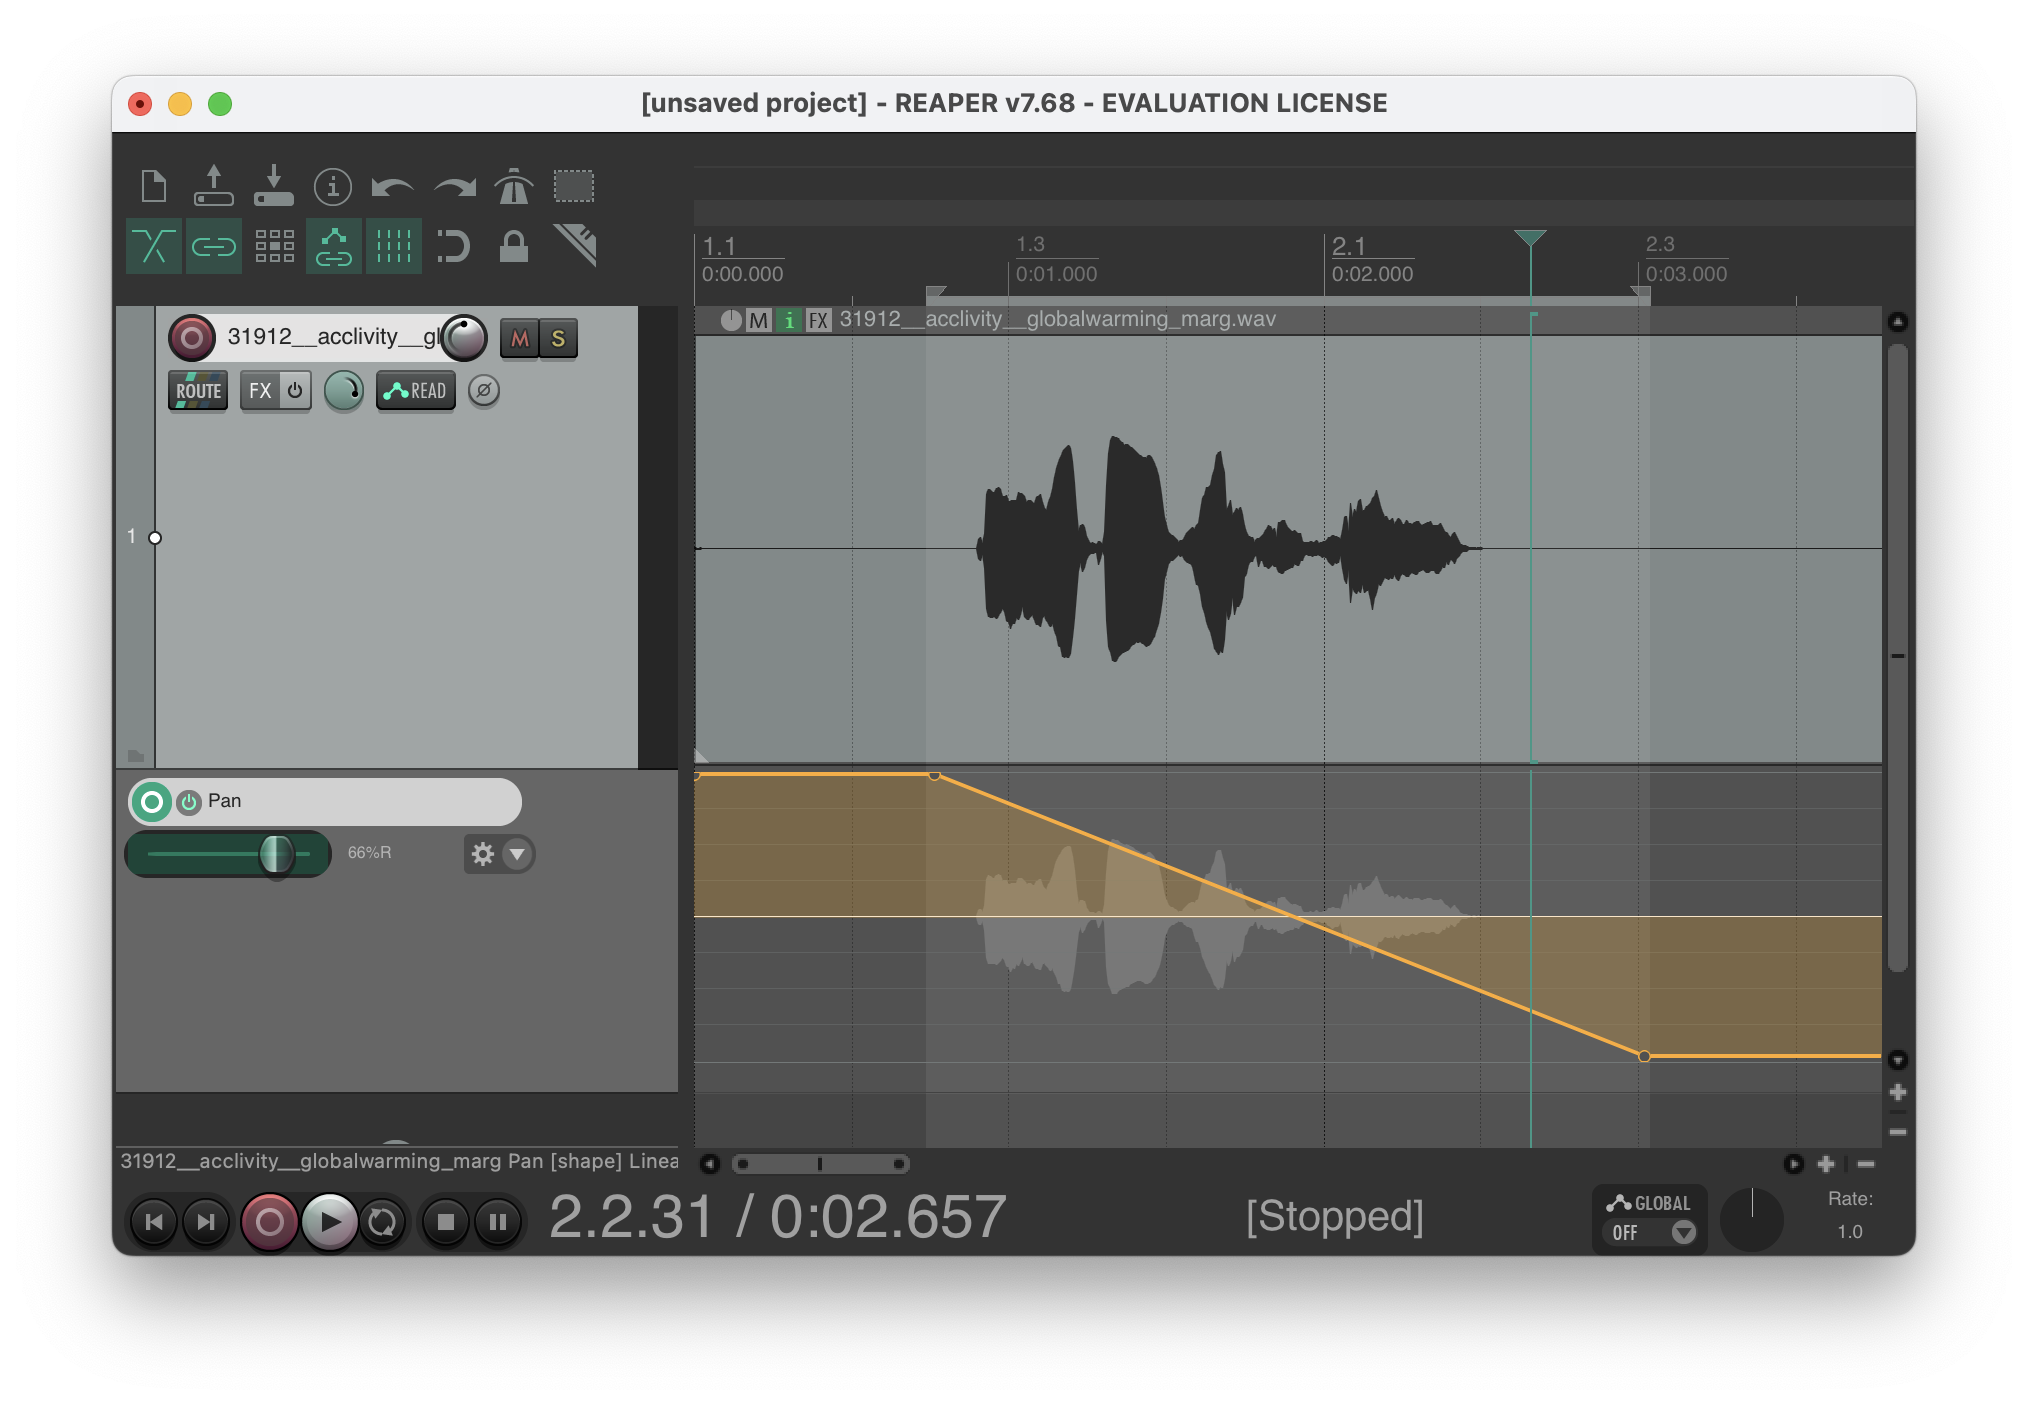
\includegraphics[width=\linewidth]{figures/daw.png}
        \caption{Recording project in the Reaper \gls{daw} \cite{REAPERAudioProduction}}
        \label{fig:daw}
    \end{subfigure}

    \bigskip
    
    \begin{subfigure}[b]{\textwidth}
        % \centering
        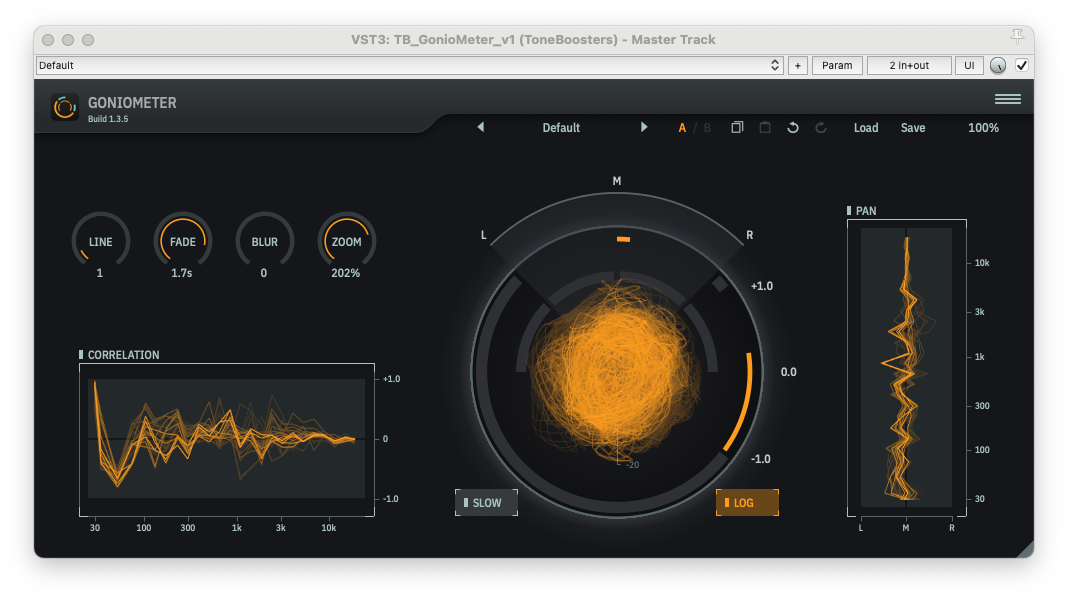
\includegraphics[width=\linewidth]{figures/goniometer_plugin.png}
        \caption{ToneBoosters Goniometer plugin \cite{ToneBoostersAudioPlugins}}
        \label{fig:goniometer}
    \end{subfigure}
    \caption{Screenshots of example music production tools}
\end{figure}

While there are some typical practices in the industry, it must again be emphasized that panning and creation of stereo field more generally is an artistic process \cite{izhakiPanning2023}. The producer pans each track individually by either physically turning the \mbox{pan-pots} or adjusting a digital panning control, and judges the stereo image purely by listening. Producers are typically known for their individual style and taste, and the ways in which they use panning in a large \gls{daw} session containing many tracks forms part of that style.

In some cases the producer consults monitoring equipment such as a level meter or goniometer to fine tune their mix \cite{ziemerAcousticFeaturesRecording2021,ziemerGoniometersArePowerful2023}. They also look for potential quality issues that can occur when the stereophonic recordings are mixed down into a monophonic signal for reproduction, which have been documented well before the advent of digital recording \cite{harveyCompatibilityProblemsTwochannel1962}. In more modern production, \gls{daw} plugins are generally used to visualize and assess the stereo qualities of the final mix \cite{bitzerSpatialDistributionMeter2007,ziemerGoniometersArePowerful2023}. \Cref{fig:goniometer} shows one example - the ToneBoosters Goniometer plugin \cite{ToneBoostersAudioPlugins}. It is designed to replicate an analogue goniometer, which, taking two voltage signals as input, displays them on a 2D axis such that a music producer might be able to discern the correlation between the signals.


\subsection{Audio representations}
Audio representations are standard paradigms that an audio recording can follow. If we consider an audio recording as a set of concurrent time signals, the representation defines how each signal in the set should be interpreted. They are usually grouped into \q{channel-based}, \q{scene-based}, and \q{object-based}. In channel-based audio, each signal represents the exact waveform that should be played back by a single loudspeaker. In scene-based and object-based audio, each signal represents one part of a larger scene, and rendering equipment is responsible for translating that scene to individual speakers \cite{sugimotoSpecificationAudioRepresentations2024}. While the focus of this thesis in on stereo audio, it is important to compare stereo to the wider audio landscape to understand why it is so heavily used for recorded music.

\subsubsection*{Monophonic}
Monophonic recordings contain a single channel to be played back on one speaker. They are only able to convey a small amount of spatial information; reverberation is the only way to infer a sense of space. Archival/historical recordings will be recorded in mono, as well as a majority of raw studio stems, speech, and telephony recordings.

\subsubsection*{Stereophonic}
Stereo recordings contain two channels: left and right. Compared to mono, stereo has the ability to convey the width and location of a sound 2D space. For music this sense of space is especially important since music signals tend to be highly dense and complex. Stereo mixing therefore allows music producers to add clarity and balance to their recordings. This marked increase in quality drove stereo's commercial adoption in the 1950s, and it has been the dominant format for recorded music since then \cite{lanierHIFITWOCHANNELCOMMOTION1957}.

\subsubsection*{Binaural}
Binaural can be considered a subset of stereo. Each channel conveys the precise sound wave as heard at the left and right ears. It is typically used when rendering spatial audio\footnote{The exact definition of \q{spatial audio} is somewhat contested in the literature but here I assume \citeauthor{cobosOverviewMachineLearning2022}'s definition: \textit{\q{audio that contains spatial information}} \cite{cobosOverviewMachineLearning2022}.} for playback on headphones, and in \gls{vr} or \gls{ar} scenarios.

\subsubsection*{Multichannel}
Multichannel is a continuation of stereo which adds speakers at more positions. While it could contain any number of channels, there are some standards that are referred to by their channel count and layout, e.g. 5.1 (5 listener-plane channels, 1 \gls{lfe} channel) or 22.2 (10 listener-plane, 2 \gls{lfe}, 9 overhead, 3 low) \cite{sugimotoSpecificationAudioRepresentations2024}. Compared to stereo, it has the ability to convey width, depth, and -- depending on the arrangement -- height, creating a higher sense of immersion. This ability sees it being used mainly for film and TV soundtracks where the emotional impact of single sound events can be critical. That said, the high setup cost and difficulty positioning extra speakers has historically discouraged its wider adoption \cite{bayleySurroundSoundDAW2012}.

\subsubsection*{Ambisonics}
Ambisonics is a scene-based audio representation where each channel is one directional component of a 3D physical sound field. Recordings are referred to by their \q{order}, which implies both the number of different directions and the number of channels. The number of required channels increases quadratically with the order according to the formula $C=(O + 1)^2$ where $C$ is the number of channels and $O$ is the order. Ambisonics typically excels at representing diffuse sounds, but struggle to represent point sources unless the order is very high. Thus, ambisonic recordings are only used for very specific types of music, such as orchestral performances in large concert halls where accurate recreation of the ambience is more important than individual instruments. Even in those cases, an ambisonic recording will generally be rendered to binaural for mass distribution \cite{churnsideAmbisonicsPeriphony2010}.

\subsubsection*{Object-based audio}
In object-based audio, the entire audio scene is composed of individual audio objects accompanied by metadata specifying their location and movement. Rendering equipment is then responsible for translating those objects to speaker channels for playback. It is a relatively new format and while its main use is for cinematic sound, the music industry has recently begun to adopt it. In contrast to ambisonic recordings, object-based audio is distributed in its original form, allowing the same set of signals to be rendered in multiple ways.
\\\\
Overall, stereo recordings are able to deliver high enough quality for the majority of music listeners. The newer formats, while gathering interest in pockets of the music community, have yet to receive wide-spread adoption from consumers. The result is that the mainstream distribution of music still happens in stereo.

\subsection{Lossless and lossy encoding}
Regardless of which audio representation is chosen, the resulting recording will most likely be encoded to a compressed format for distribution. There are two types of compression: \q{lossless} and \q{lossy}. A lossless format, when decoded, will produce bit-for-bit recreation of the input signal. Lossy formats on the other hand will not produce the exact same signal, but will discard information that they consider irrelevant according to a psychoacoustic model. There are many lossy formats each suitable for different types of audio, but for the purposes of this thesis it is just pertinent that spatial information can be lost during lossy encoding.

% \clearpage

\section{Analysis of digital recordings}

The output of a recording session is usually only the stereo mix. Stems and \gls{daw} sessions are generally kept private, with precious few being available under licensing terms that are conducive to academic research \cite{bittnerMedleyDBMultitrackDataset2014}. Thus, we assume that all analysis can only be performed on the final stereo mixes that are distributed for playback. The most common distribution format is a digital audio file, and there are some fundamental analysis techniques that can be applied to a digital audio signal.

\subsection{Digital audio signals}
When a sound wave interacts with a microphone, it generates an electrical signal in continuous time. To convert that analogue signal into a digital one, it is sampled at regular intervals. The sampling frequency ($f_s$) is related to the sampling interval ($T_s$) by the relationship $T_s = \frac{1}{f_s}$.

Shannon's sampling theorem states that a signal can be perfectly recreated when sampled at twice the highest frequency contained in the signal. Conversely, the highest frequency that can be represented by sampling a signal at a given $f_s$ is half of that frequency. This limit is called the \q{Nyquist frequency} and is calculated by $f_N = \frac{f_s}{2}$ \cite{yaoNyquistFrequency1983}. This is illustrated by \Cref{fig:nyquist}, which shows the sampling of three waveforms. The lower plot shows a signal at the Nyquist frequency ($f_N$), which can be perfectly reconstructed from the digital samples. The upper two waveforms have frequencies equidistant but in opposite directions from the Nyquist frequency ($f_N \pm f_{\delta}$). The digital samples shown in circles could represent either of the two waveforms. In practice, when the analogue waveform is reconstructed, the lower frequency will always take precedence. 

\begin{figure}[t!]
    \centering
    \includegraphics{nyquist.pdf}
    \caption{Illustration of the Nyquist Frequency in digital audio signals. Dotted vertical lines represent sampling points with a separation of $T_s$, and monotonically increasing index $n$. The upper plot shows a cosine wave at exactly $f_N$. The lower plot shows two cosine waves with frequencies equidistant above and below the Nyquist frequency ($f_N$). Sampled values are shown as circle marks on the plots. The two upper signals can both be represented by same digital samples.}
    \label{fig:nyquist}
\end{figure}

A typical $f_s$ for music is \qty{44.1}{\kHz}, with a resulting $f_N$ of \qty{22.05}{\kHz}. The prevalence of this particular number stems from the first widespread distribution mechanism for digitally encoded music - the \gls{cd}\footnote{\qty{44.1}{\kHz} was chosen by a consortium of \gls{cd} manufacturing companies as a trade-off between technical requirements and the limits of human perception \cite{baertDigitalAudioCompact2013}.}. While higher frequencies may be used in the recording and production process, an exceedingly large proportion of recorded music has been distributed at \qty{44.1}{\kHz}, even after \glspl{cd} were displaced by other distribution methods.

\subsection{Time-Frequency representation of audio}

In order to perform many types of audio analysis, the audio signal can be converted from the time domain into the \gls{tf} domain. In perceptual acoustics research there are several common forms of \gls{tf} representation, each with its own nuances. This section provides those details, and a side-by-side comparison is shown at the end of the section in \cref{fig:spect_comp}.

\subsubsection{\gls{stft} spectrogram}

The \gls{stft} spectrogram is one of the most popular \gls{tf} representions across all audio processing work due to its computational efficiency. The fundamental principle is that a time-domain signal is split into short (1 to 100ms) overlapping chunks, and the \gls{fft} is performed on each chunk, thereby converting that chunk into the frequency domain.  By arranging subsequent frames along a time axis it is possible to represent the original signal as a 2D image known as a spectrogram. When the time-domain signal is entirely real, (which is the case for monophonic audio signals), the result of the \gls{fft} will be a complex signal which is symmetrical around the Nyquist frequency and the upper half is therefore dropped. Furthermore, the complex spectrum is usually represented in magnitude/phase form to better match the human auditory response.

A fundamental property of the \gls{fft} is that it assumes that the signal repeats outside the time frame that is being analysed. Since this is generally not the case for audio signals, it is standard practice to apply a time-domain windowing function to each frame so that large transients do not occur at the boundaries. Several standard windowing functions exist, each with their own nuances, but for most audio applications the \q{Hann} window can be used \cite{LibrosastftLibrosa0110}. 

The nature of the spectrogram is affected by two parameters: the frame size and hop size. \q{Frame size} refers to the number of samples in each analysis frame. To obtain maximal computational efficiency this must be a power of 2. \q{Hop size} refers to the number of samples between the start of subsequent frames and is sometimes expressed as a percentage of the frame size. The frame size dictates the resolution of the spectrogram's frequency axis since the frequency bins will be spaced evenly between \SI{0}{\hertz} and the Nyquist frequency. Importantly, a longer frame size will result in lower time accuracy within each frame; sharp transients in the time domain will appear as wideband energy in the frequency domain, but information about exactly where the transient occurred within the frame is lost. To counteract this inaccuracy, a smaller hop size can be used so that transients might be detected as sharp changes between \gls{stft} frames. One major drawback of the \gls{stft} spectrogram is that the linearly-spaced frequency bins do not align well with the human perception of frequency, which is logarithmic. The \gls{stft} therefore contains redundant information in higher frequencies. Several common alternatives exist to account for this.

\begin{figure}[htb]
    \centering
    \includegraphics{stft_spect.pdf}
    \caption{\gls{stft} spectrogram of a speech recording.}
    \label{fig:stft_spect}
\end{figure}

\subsubsection{Mel spectrogram}

The \q{Mel scale} is a quasi-logarithmic frequency scale derived from perceptual experiments. Several definitions exist in the literature \cite{umeshFittingMelScale1999}, but popular implementations like that of librosa \cite{mcfeeLibrosaAudioMusic2015} and \gls{amt} \cite{majdakAMT1xToolbox2022} tend to underpin most audio experimentation.

A \q{Mel filter bank} is a set of band-pass filters that are spaced equally on the Mel scale. Practically, they are implemented as sets of weights that are applied to an \gls{stft} spectrum with the relationship $M_n = \sum_{k=0}^{N} S_k W_{k,n}$ where $M_n$ is the $n$th Mel coefficient, $S_k$ is the $k$th \gls{stft} bin, $N$ is the number of \gls{stft} bins, and $W_{k,n}$ is the $k$th weight of the $n$th Mel filter. An example Mel filter bank with 8 filters is shown in \cref{fig:mel_filters}. While 8 filters are shown for demonstration purposes, audio analysis typically requires over 100. When this filter bank is applied to each time step of an \gls{stft} spectrogram, the result is a \q{Mel spectrogram}, an example of which can be seen in \cref{fig:mel_spect}. Observe that the higher frequencies have been condensed into fewer frequency bins compared to the \gls{stft} spectrogram.


\begin{figure}[b!]
    \centering

    \begin{subfigure}[h]{\textwidth}
        \centering
        \includegraphics{mel_filterbank.pdf}
        \caption{Example Mel filter bank containing 8 filters, shown with linear (left) and logarithmic (right) frequency scales. The bandwidth of each filter is roughly equal in logarithmic space, and the amplitudes are scaled so that the sum of the weights in each band is equal. Filter weights equal to zero are removed for clarity. 
        % The filters are calculated using librosa \cite{LibrosafiltersmelLibrosa0110} using a sample rate of \SI{44100}{\hertz} and an \gls{fft} size of 4096 samples.
        }
        \label{fig:mel_filters}
    \end{subfigure}

    \bigskip

    \begin{subfigure}[h]{\textwidth}
        \centering
        \includegraphics{mel_spect.pdf}
        \caption{Mel spectrogram of a speech recording, using 32 bands.}
        \label{fig:mel_spect}
    \end{subfigure}
\end{figure}

\subsubsection{Cochleagram}

As an alternative to the two spectrogram representations, a cochleagram aims to make a \gls{tf} representation that models the acoustic response of the human cochlea more closely. To that end, all processing is performed in the time domain and is sometimes referred to as a \q{peripheral ear model}. Several examples appear in the literature \cite{boddenBinauralModelingAuditory1995,choiObjectiveMeasurementPerceived2008,delgadoDesignChoicesBinaural2023}. In the classical method \cite{boddenBinauralModelingAuditory1995} the original signal is first processed by a bank of gammatone filters with their centre frequencies placed according to a perceptual scale (such as the \gls{erb} scale \cite{smithiiiEquivalentRectangularBandwidth2020}), as shown in \cref{fig:gammatone_filters}. As with Mel filters, several definitions of gammatone filters exist in the literature, but the popular implementations (e.g. scipy \cite{virtanenSciPy10Fundamental2020} and \gls{amt} \cite{majdakAMT1xToolbox2022}) preside. \Cref{fig:cochleagram} shows a cochleagram of the example speech recording.

\Cref{fig:cochleagram_steps} shows the intermediate steps to generate a cochleagram. Each sub-band signal is processed by a half-wave rectifier, square root, and low-pass filter to mimic the excitation patterns of the cilia and basilar membrane. The result is a signal representing the envelope of each sub-band. Those envelopes are then segmented into overlapping time chunks. The amplitude of each chunk is then calculated as the mean of all its values, forming one pixel in the cochleagram.

\begin{figure}[hbt]
    \centering
    \includegraphics{cochleagram.pdf}
    \caption{Cochleagram of a speech recording, using 32 bands.}
    \label{fig:cochleagram}
\end{figure}

\begin{figure}[p!]
    \centering
    \begin{subfigure}[b]{0.8\textwidth}
        \centering
        \includegraphics{gammatone_filterbank.pdf}
        \caption{Example gammatone filter bank with individual filters spaced equally on the \gls{erb} scale. The filters are \glsentryfull{iir} and are applied to an audio signal in the time domain.}
        \label{fig:gammatone_filters}
    \end{subfigure}

    \begin{subfigure}[b]{\textwidth}
        \includegraphics{cochleagram_steps.pdf}
        \caption{Steps of an example decomposition from time-domain audio to a cochleagram. The audio being filtered is a frequency sweep from 100 to 20000 Hz. First it is processed by a gammatone filter bank, generating 8 sub-band signals which are spaced equally on the \gls{erb} scale. Each sub-band has its envelope extracted. The envelope is then split into overlapping time chunks, which are averaged to form the cochleagram.}
        \label{fig:cochleagram_steps}
    \end{subfigure}
    \caption{Using a gammatone filter bank to make a cochleagram.}
\end{figure}


\begin{figure}[p!]
    \centering
    \includegraphics{spect_comp.pdf}
    \caption{An example audio signal displayed as \gls{stft} spectrogram (above), Mel spectrogram (mid), and cochleagram (below). The spectrogram frequency bands are spaced linearly between 0Hz and the Nyquist frequency, which is not coherent with human perception. The Mel spectrogram is created from the original spectrogram based on linear combinations of its frequency bands and retains more detail in lower frequencies than higher frequencies. The Cochleagram is created directly from time domain audio by mimicking the physical response of the human ear.}
    \label{fig:spect_comp}
\end{figure}

\pagebreak

\subsection{Machine learning}
Any data-driven audio research, particularly that using vast datasets, will naturally involve the use of \gls{ml}. Broadly speaking, \gls{ml} techniques can be classified as either supervised or unsupervised. When training a supervised  \gls{ml} model, the training dataset needs to include ground-truth labels such that the network can objectively discern via a loss function whether the predictions it is making are correct. Unsupervised \gls{ml} on the other hand does not require any labels. Instead, it seeks to form a representation of the underlying dataset via techniques such as clustering or dimensionality reduction, thereby learning the structures and patterns of the data while retaining as much key information as possible.

Striking a middle ground between the two is \q{self-supervised} learning, which addresses the issue of creating objective ground-truths from unlabelled data. Instead of relying on external labels, self-supervised learning generates pseudo-labels from the dataset itself, and then uses those as the input to a \q{pretext task}, which is tackled in much the same way as a supervised task.

As an example we can consider the current largest dataset of recorded music: \gls{fma} \cite{defferrardFMADatasetMusic2017}. The dataset contains the stereo audio of approximately \num{100000} tracks, along with metadata such as genre tags. An unsupervised task might involve learning a high-order representation of the raw spatial cues present in the stereo signals. A supervised task might involve predicting genre using the audio signal as input. A self-supervised task might involve masking off a short period of audio and filling it back in using the surrounding audio as context. 

In relation to the \hyperref[sec:research_questions]{overarching \gls{rq}} in \cref{sec:research_questions}, we assume that a music producer's \gls{daw} session is the only source of objective ground-truth data regarding stereo field. Furthermore, we assume that \gls{daw} sessions are not publicly available, as was found in \cite{colonelReverseEngineeringRecording2021,rodriguezSpectralDynamicConstellations2024}; The only public-facing output of a recording session is the mixdown. It follows that either unsupervised or self-supervised learning is necessary to draw any conclusions to the \glspl{rq}.



